\section{Introduction}\label{sec:intro}

Objects in the real world rarely exist in isolation; 
% understanding and 
modeling the relationships between them is essential to accurately capturing complex systems. As increasingly powerful machine learning models progress towards building internal ``world models,'' it is important to explore natural inductive biases to enable efficient learning of relational representations. The computational challenge lies in developing the components necessary for constructing robust, flexible, and progressively complex relational representations.

Compositionality---used here to mean an ability to compose modules together to build iteratively more complex feature representations---is essential to the success of deep representation learning. 
% For example, in a feedforward network, each layer builds on the one before, and in a CNN, each convolution builds an iteratively more complex feature map~\citep{zeiler2014visualizing}. 
For example, CNNs extract higher-level features (e.g., textures and object-specific features) by composing simpler feature maps~\citep{zeiler2014visualizing}, resulting in a flexible architecture for computing ``features of features''.
So far, work on relational representation learning has been limited to ``flat'' first-order architectures. In this work, we propose \textit{\bfseries relational convolutional networks} as a compositional framework for learning hierarchical relational representations.

\begin{wrapfigure}{R}{0.5\textwidth}
    \centering
    \vskip-12pt
    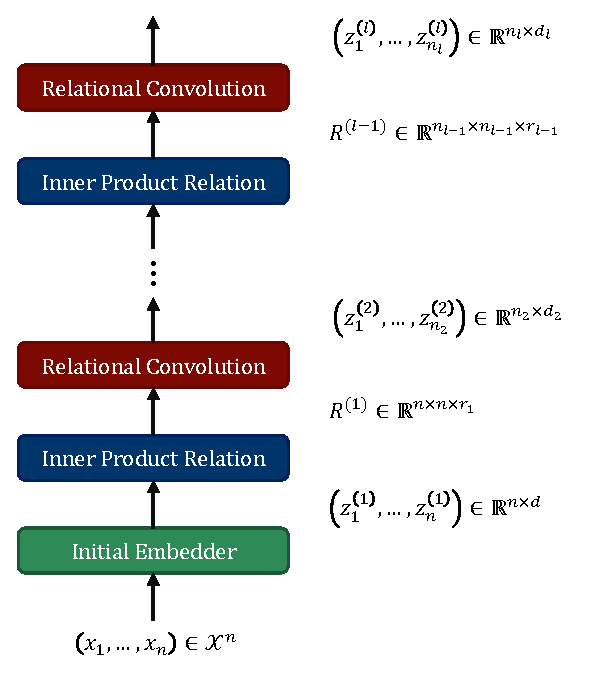
\includegraphics[width=.48\textwidth]{figs/relconv_architecture.pdf}
    \vskip-12pt
    \caption{Proposed architecture for relational convolutional networks. Hierarchical relations are modeled by iteratively computing pairwise relations between objects and convolving the resultant relation tensor with graphlet filters representing templates of relations between groups of objects.
    }\label{fig:relconv_architecture}
    % \vskip-12pt
\end{wrapfigure}

The key to the framework proposed in this paper involves formalizing the concept of convolving learnable templates of a relational pattern against a larger relation tensor. This operation produces a sequence of vectors representing the relational pattern within each group of objects. Crucially, composing relational convolutions captures higher-order relational features---i.e., relations between relations. Specifically, our proposed architecture introduces the following novel concepts and computational mechanisms.
\begin{itemize}%[itemsep=1pt]
    \item \textit{\bfseries Graphlet filters.} A ``graphlet filter'' is a template for the pattern of relations between a (small) collection of objects. 
    Since pairwise relations can be viewed as edges on a graph, the term ``graphlet'' is used to refer to a subgraph, and the term ``filter'' is used to refer to a learnable template or pattern.
    % Graphlet filters are analogous to filters (also called kernels) in traditional CNNs for images, which represent templates for local regions of an image.
    \item \textit{\bfseries Relational convolutions.} 
    We formalize a notion of \textit{relational} convolution, analogous to spatial convolutions in CNNs, where a graphlet filter is matched against the relations within \textit{groups} of objects to obtain a representation of the relational pattern in different groupings of the input.
    % In CNNs for image processing, each filter is
    %  ``swept,'' or 
    % spatially convolved across the image. For relational learning, we formalize an analogous notion of convolution where a graphlet filter can be matched against the relations between each group of objects.
    \item \textit{\bfseries Grouping mechanisms.} For large problem instances, it would be computationally and statistically intractable to consider relational convolutions across all combinations of objects. To achieve scalability, we introduce a learnable grouping mechanism based on attention which identifies the relevant groups that should be considered for the downstream task.
    \item \textit{\bfseries Compositional relational modules.} The proposed architecture supports composable modules, where each module has learnable graphlet filters and groups. This enables learning higher-order relationships between objects---relations between relations.
\end{itemize}


The architecture is presented in detail in Sections~\ref{sec:mdipr} and~\ref{sec:relconv}, and a schematic of the proposed architecture is shown in~\Cref{fig:relconv_architecture}. In a series of experiments, we show how relational convolutional networks provide a powerful framework
% and inductive bias 
for relational learning. We first carry out experiments on the ``relational games'' benchmark for relational reasoning proposed by~\citet{shanahanExplicitlyRelationalNeural}, which consists of a suite of binary classification tasks for identifying abstract relational rules between a set of geometric objects represented as images. 
We next carry out experiments on a version of the \textit{Set} game, which requires processing of higher-order relations across multiple attributes. We find that relational convolutional networks outperform Transformers, graph neural networks, as well as existing relational architectures. These results demonstrate that both compositionality and relational inductive biases are needed to efficiently learn representations of complex higher-order relations.

\subsection{Related Work}\label{ssec:related_work}

To place our framework in the context of previous work, we briefly discuss related forms of relational learning below, pointing first to the review of relational learning inductive biases by~\cite{battagliaRelationalInductiveBiases2018}%,palmRecurrentRelationalNetworks2018,zhangRAVENDatasetRelational2019}. % battaglia is a review of "relational inductive biases" (though in a somewhat different sense to us). the rest are more specific, so this may not be the best place to cite them.

{Graph neural networks} (GNNs) are a class of neural network architectures which operate on graphs and process ``relational'' data~\citep[e.g.,][]{niepertLearningConvolutionalNeural2016,kipfSemiSupervisedClassificationGraph2017,schlichtkrullModelingRelationalData2017,velickovicGraphAttentionNetworks2017,kipfNeuralRelationalInference2018,xuHowPowerfulAre2018}. A defining feature of GNN models is their use of a form of neural message-passing, wherein the hidden representation of a node is updated as a function of the hidden representations of its neighbors on a graph~\cite{gilmerNeuralMessagePassing2017}. Typical examples of tasks which GNNs are applied to include node classification, graph classification, and link prediction~\cite{hamiltonGraphRepresentationLearning2020}. %This is a very general model which includes as a special case convolutional neural networks, where the graph is a grid, and Transformers, where the graph is a complete graph and the message-passing function is a convex sum of the neighbors' representations.

In GNNs, the `relations' are given to the model via edges in a graph. In contrast, our architecture, as well as the explicitly relational architectures described below, operate on collections of objects without any relations given as input. Instead, such relational architectures must infer the relevant relations from the objects themselves. Still, graph neural networks can be applied to these relational tasks by passing in the collection of objects along with a complete graph. % A Transformer Encoder can be thought of as a special case of this architecture.%, and hence is the representative baseline we compare against in our experiments.

Several works have proposed architectures with the ability to model relations by incorporating an {attention mechanism}~\citep[e.g.,][]{vaswani2017attention,velickovicGraphAttentionNetworks2017,santoroRelationalRecurrent2018,zambaldiDeepReinforcementLearning2018,locatelloObjectCentricLearningSlot2020}. Attention mechanisms, such as self-attention in Transformers~\citep{vaswani2017attention}, model relations between objects implicitly as an intermediate step in an information-retrieval operation
% a form of neural message-passing in order 
to update the representation of each object as a function of its context.

There also exists a growing literature on neural architectures which aim to explicitly model relational information between objects. An early example is the relation network proposed by~\citet{santoroSimpleNeural2017}.~\citet{shanahanExplicitlyRelationalNeural} proposes the PrediNet architecture, which aims to learn relational representations which are compatible with predicate logic.
% \todo{removed citation of ESBN for space (since not in baselines). can put back in camera-ready.}
% ~\citet{webbEmergentSymbols2021} proposes ESBN, a recurrent neural network augmented with external memory whose memory-write operation aims to factors representations into `sensory' and `relational'.
~\citet{kergNeuralArchitecture2022} proposes CoRelNet, a simple architecture based on `similarity scores' which aims to distill the relational inductive biases discovered in previous work into a minimal architecture.~\citet{altabaaAbstractorsTransformer2023} explored relational inductive biases in the context of Transformers, and proposed a view of relational inductive biases as a type of selective ``information bottleneck'' which disentangles relational information from object-level features.~\citet{webbRelationalBottleneckInductive2023} provides a cognitive science perspective on this idea, arguing that a relational information bottleneck may be a mechanism for abstraction in the human mind.% and brain.

